\begin{wrapfigure}{r}{0.3\textwidth}
  \begin{center}
  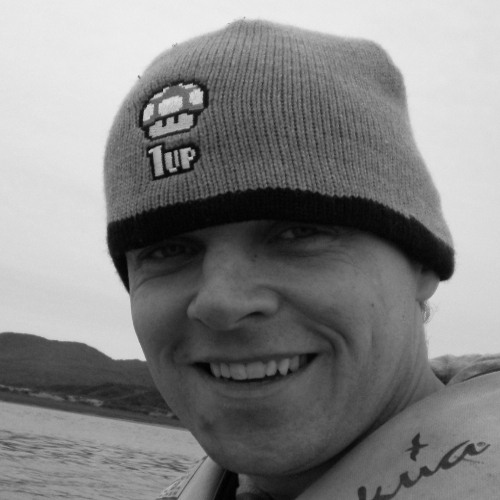
\includegraphics[width=3cm]{fig/avatar-miekg-300x300}
  \end{center}
\end{wrapfigure}
Miek Gieben has a master's degree in Computer Science from the Radboud University Nijmegen (Netherlands).
He is involved in the development and now the deployment of the DNSSEC protocol \cite{RFC4033,RFC4034,RFC4035} --
the succesor of the DNS and as such co-authored \cite{RFC4641}.
After playing with the language Erlang, Go was the first concurrent language
that actually stuck with him.
He fills his spare time with coding in, and writing of Go. He is the maintainer
of the Go DNS library: \url{https://github.com/miekg/godns}.
He maintains a personal blog on \url{http://www.miek.nl} and tweets
under the name \texttt{@miekg}. The postings and tweets may sometimes 
actually have to do something with Go.
